\section{Combat Techniques}

Combat techniques are special maneuvers that you can perform while in combat, allowing you to do more than just move and swing a weapon. Combat techniques generally require an action to execute and cost stamina. Techniques labeled as "Reaction" can be executed in response to a specific event instead of using an action on your turn. Each reaction technique imposes an additional penalty die on the next one until your next turn. For example, if you have dodged and fought back between turns, attempting to dodge again will be an Acrobatics check with two penalty dice (in addition to any that may be imposed by other circumstances).

\subsection{Common Techniques}

While certain combat techniques will only be available to skilled warriors while wielding specific weapons, some techniques are available to everyone and can be used with various different weapons.

\begin{itemize}
	\item \textbf{Block} (\textit{10 Stamina, Reaction}): If you are targeted by a melee attack, you may attempt to block it. Make an opposed Block check. On a success, you block the attack and take no damage.
	\item \textbf{Dive for Cover} (\textit{Free, Reaction}): When you first notice an enemy, you may dive for the ground as a reaction, preferably behind cover. Otherwise, this technique costs an Action. You are able to cover 10 feet using this move, and you go prone as a result. This move imposes a penalty on ranged attack rolls targeting you.
	\item \textbf{Dodge} (\textit{10 Stamina, Reaction}): If you are targeted by a melee attack, you may attempt to dodge by making an opposing Acrobatics check. On a success, you dodge the opponent's attack entirely and take no damage. On a tie, the dodger wins.
	\item \textbf{Dual Wield Attacks} (\textit{Free, Bonus Action}): If you attack with a light, one-handed weapon and are holding another light, one-handed weapon, you may attack with the latter as a bonus action; however, the second attack does not benefit from your damage bonus. If you use Flurry of Blows while dual wielding, each weapon gets only two attacks, for a total of four. The damage bonus rule still applies to your off-hand weapon in this case.
	\item \textbf{Fight Back} (\textit{10 Stamina, Reaction}): You respond to incoming melee attacks with attacks of your own. You must be within range of the attacker and not otherwise unable to attack. You can only make one attack, it may not be a combat technique. On a success, you avoid coming to harm and your attacker suffers damage. On a tie or failure, your attack fails to land and your attacker successfully strikes you.
	\item \textbf{Flurry of Blows} (\textit{60 Stamina, Action}): You swing your weapon(s) quickly, dealing multiple blows in a single round. Light weapons may attack 3 times, medium weapons may attack twice, and heavy weapons may not use this technique. For the purpose of successive reaction penalty dice, this technique counts as one attack.
	\item \textbf{Grapple} (\textit{20 Stamina, Action}): If you have at least one free hand, you may attempt to grab your target. Make a melee attack using your Athletics skill. You do no damage, but the target is grappled on a success. A grappled target cannot move. Your speed while holding an unwilling creature is halved. A grappled creature may attempt to break free with its action using an opposed Athletics check.
	\item \textbf{Opportunity Attack} (\textit{10 Stamina, Reaction}): If a combatant leaves your melee range during their turn, you may react by making a single attack against them.
	\item \textbf{Sneak Attack} (\textit{Free, Action}): If you are undetected, you may attack a target for bonus damage determined by your Sneak skill (\textit{see section 3.2}). Sneak attacks always gain a bonus die, but their damage multipliers do not stack with those of other combat techniques.
\end{itemize}

\subsection{Weapons \& Skill-Based Combat Techniques}

The following sections describe different types of weapons and the combat techniques associated with that weapon type. Please note that the weapon types listed are merely types and not specific weapons; while all weapons of that type you find in the game will have the listed properties, some features might vary. Also, for every melee technique listed in this section, the following applies: if your target successfully rolls to block your attack and you used a light weapon to make it, the target is recoiled.

\subsubsection{Blade}

Bladed weapons are deadly in the hands of highly skilled wielders thanks to their \textit{Impaling} property. They tend to be more effective against poorly armored opponents thanks to the ease with which blades can cut through flesh compared to the effects of blunt weapons. Bladed weapons in the Elder Scrolls Tabletop RPG come in four varieties:

\begin{itemize}
	\item \textbf{Daggers} (\textit{1d6, Light, One-Handed}): Blades shorter than the forearm. Not very effective against armor, but incredibly deadly in the hands of an adept sneak.
	\item \textbf{Shortswords} (\textit{1d8, Light, One-Handed}): Short, thin bladed swords. More effective than daggers in open combat, but less optimal for sneak attacks.
	\item \textbf{Longswords} (\textit{1d10, Medium, One-Handed}): Long, somewhat heavy blades designed for one- or two-hand grips. Not as quick as a shortsword or dagger, but weighty enough to fare well against armor.
	\item \textbf{Claymores} (\textit{2d6, Heavy, Two-Handed, Reach}): Very long and heavy blades that must be wielded with two hands in order to use them effectively. Great for heavy combat and punching holes in armor at the cost of slow swings.
\end{itemize}

Blade techniques are primarily focused on dealing as much damage as possible. They become available every 25 skill points in Blade as specified in the mastery perk table (\textit{section 3.2}). Each of these techniques costs 60 stamina to execute. If a target successfully blocks a blade technique you made with a medium or heavy blade, they receive recoil. Thus, even failing to land these big hits can come with some benefits. The five blade techniques are:

\begin{itemize}
	\item \textbf{Power Attack}: You wind up and unleash a heavy blow, doubling your damage.
	\item \textbf{Standing Strike}: You plant your feet and strike with all your might, tripling your damage at the cost of being unable to move on the same turn.
	\item \textbf{Flanking Strike}: You swing your weapon broadly across the area in front of you, doubling your damage and allowing you to attack two adjacent targets within reach. (You only roll attack once; each target rolls block/dodge against that number, and attacks are resolved individually.)
	\item \textbf{Sweeping Attack}: You aim low, attempting to strike at your opponent's legs. Damage is doubled; on an extreme success, your opponent is knocked prone.
	\item \textbf{Dizzying Blow}: You swing directly for your opponent's head. Damage is doubled. On an extreme success, your opponent is paralyzed until the end of their next turn.
\end{itemize}

\subsubsection{Blunt}

In general, blunt weapons are more effective against armor due to the manner in which they bludgeon weak points. However, they do not get the \textit{Impaling} bonus to extreme successes; instead, they merely deal max damage. There are four types of blunt weapons:

\begin{itemize}
	\item \textbf{War Axes} (\textit{1d8, Light, One-Handed}): Hand-sized axes, light and quick for blunt weapons. Their weight makes them better at penetrating armor than other light weapons.
	\item \textbf{Maces} (\textit{1d10, Medium, One-Handed}): Bludgeons with a weighty head at the end of a handle. Useful for crumpling skulls and armor alike. Not quite as swift as war axes, but significantly more effective against armored foes.
	\item \textbf{Battleaxes} (\textit{1d12, Heavy, Two-Handed, Reach}): Big, heavy axes that require both hands to swing. Great for cleaving limbs and leaving deep,  grievous wounds.
	\item \textbf{Warhammers} (\textit{2d6, Heavy, Two-Handed, Reach}): Huge hammers intended not for construction but smashing foes. Allows for consistently forceful strikes.
\end{itemize}

Blunt techniques are identical to Blade techniques, except they become available via advancement in the Blunt skill. Again, each technique costs 60 stamina to execute, and if a target successfully blocks one of these attacks made with a medium or heavy weapon, they receive recoil. The five blunt techniques are:

\begin{itemize}
	\item \textbf{Power Attack}: You wind up and unleash a heavy blow, doubling your damage.
	\item \textbf{Standing Strike}: You plant your feet and strike with all your might, tripling your damage at the cost of being unable to move on the same turn.
	\item \textbf{Flanking Strike}: You swing your weapon broadly across the area in front of you, doubling your damage and allowing you to attack two adjacent targets within reach. (You only roll attack once; each target rolls block/dodge against that number, and attacks are resolved individually.)
	\item \textbf{Sweeping Attack}: You aim low, attempting to strike at your opponent's legs. Damage is doubled; on an extreme success, your opponent is knocked prone.
	\item \textbf{Dizzying Blow}: You swing directly for your opponent's head. Damage is doubled. On an extreme success, your opponent is paralyzed until the end of their next turn.
\end{itemize}

\subsubsection{Hand-to-Hand Techniques}

Unarmed attacks deal less damage than blade, blunt and marksman weapons. They do not benefit from the Impaling property, nor do they get to ignore armor points like blunt weapons. They also deal less base damage than any of the listed weapons (\textit{1d4}) and do not have benefit from weapon quality damage bonuses. However, hand-to-hand attacks have the unique benefit of exhausting the target. Whenever you deal damage with an unarmed attack, half of that damage is also removed from the target's stamina. Unarmed attacks also count as light weapons and so benefit from Flurry and dual wielding. Hand-to-Hand techniques are similar to melee weapon techniques, but they are more focused on disrupting the enemy. Like the previous categories, each technique listed here costs 60 stamina to execute.

\begin{itemize}
	\item \textbf{Power Attack}: You wind up and unleash a heavy blow, doubling your damage.
	\item \textbf{Standing Strike}: You plant your feet and strike with all your might, tripling your damage at the cost of being unable to move on the same turn.
	\item \textbf{Disarming Attack}: You strike viciously at your opponent's weapon arm. Your attack deals double damage, and the opponent is disarmed on an extreme success.
	\item \textbf{Paralyzing Palm}: You strike at your opponent's vitals, causing them to reel in pain. Your attack deals double damage, and on an extreme success, the opponent is paralyzed until the end of their next turn.
	\item \textbf{Power Within}: You channel your inner power and strike a powerful blow against your foe. Your damage is doubled. On an extreme success, you may convert half of your damage to fire, frost or shock damage, your choice.
\end{itemize}

\subsubsection{Archery}

Bows are silent and lethal ranged weapons. Bows are often favored by stealthy characters as a way to attack enemies at range with minimal risk of exposure. Their ability to deliver poisons via arrowhead makes them especially potent; even if the arrow does not finish the job, the poison may. While blades can be poisoned and are still highly useful for this purpose, quite a bit of mischief can be caused when one is not within arm's reach. Poisons aside, bows are very precise puncturing weapons. While they are not as effective against armor as blunt weapons, they are highly deadly in the hands of trained archers. All bows in the ESTRPG have the \textit{Impaling} and \textit{Two-Handed} properties, since their arrows are sharp and pointed and bows take both hands to use. Just make sure you bring enough arrows with you! There are two types of bows in the game:

\begin{itemize}
	\item \textbf{Shortbows} (\textit{2d6, 80 ft, Medium}): Bows of modest length, generally allowing for faster draw speed at the cost of less power.
	\item \textbf{Longbows} (\textit{2d8, 150 ft, Heavy}): Bows typically as tall as the archer, with enough power to send arrows flying faster and farther at the cost of slower draw speeds.
\end{itemize}

Marksman attacks in combat use different mechanics from melee attacks; targets cannot react by dodging or blocking. Instead, a difficulty is chosen for the attack roll based on how far away the target is in relation to the weapon's base range (normal for within, hard for within double, extreme for within triple). Bonus and penalty dice are then assigned based on conditions affecting the shot. The conditions are as follows:

\begin{center}
\begin{tabular}{p{0.5\textwidth}p{0.5\textwidth}}
	Bonus
	\begin{itemize}
		\item Aiming
		\item Large target
	\end{itemize}
	&
	Penalty
	\begin{itemize}
		\item Small target
		\item Target is within melee range
		\item Target in partial cover
		\item Target diving for cover
		\item Firing into a melee with friendlies
		\item Fast-moving target (moved 50 feet or more on last turn)
	\end{itemize}\\
\end{tabular}
\end{center}

These apply to ranged attacks with any weapon or spell.\\

Marksman techniques are less concerned with dealing extra damage and more with improving archery conditions. Nonetheless, they typically do improve upon the already formidable base damage of bows.

\begin{itemize}
	\item \textbf{Aim} (\textit{10 Stamina}): By staying still for a round and taking no damage, you are able to concentrate and line up a good shot. Your next attack has a bonus die and +20 ft to base range.
	\item \textbf{Volley} (\textit{60 Stamina}): You can fire two arrows in one round when using a shortbow.
	\item \textbf{Trick Shot} (\textit{60 Stamina}): Your attack deals double damage and ignores penalty dice imposed by partial cover.
	\item \textbf{Focus Shot} (\textit{60 Stamina}): Your attack deals double damage and ignores penalty dice imposed by firing into a melee.
	\item \textbf{Snipe} (\textit{60 Stamina}): Your attack deals triple damage, and base range is increased by 25\% for this attack. Range bonus does not stack with Aim.
\end{itemize}

\begin{tcolorbox}
\textbf{Note}: You have a limited number of arrows, so be careful with your attacks. It is assumed you are able to recover all your arrows after combat unless something happens to them.
\end{tcolorbox}

\begin{figure}[h]
	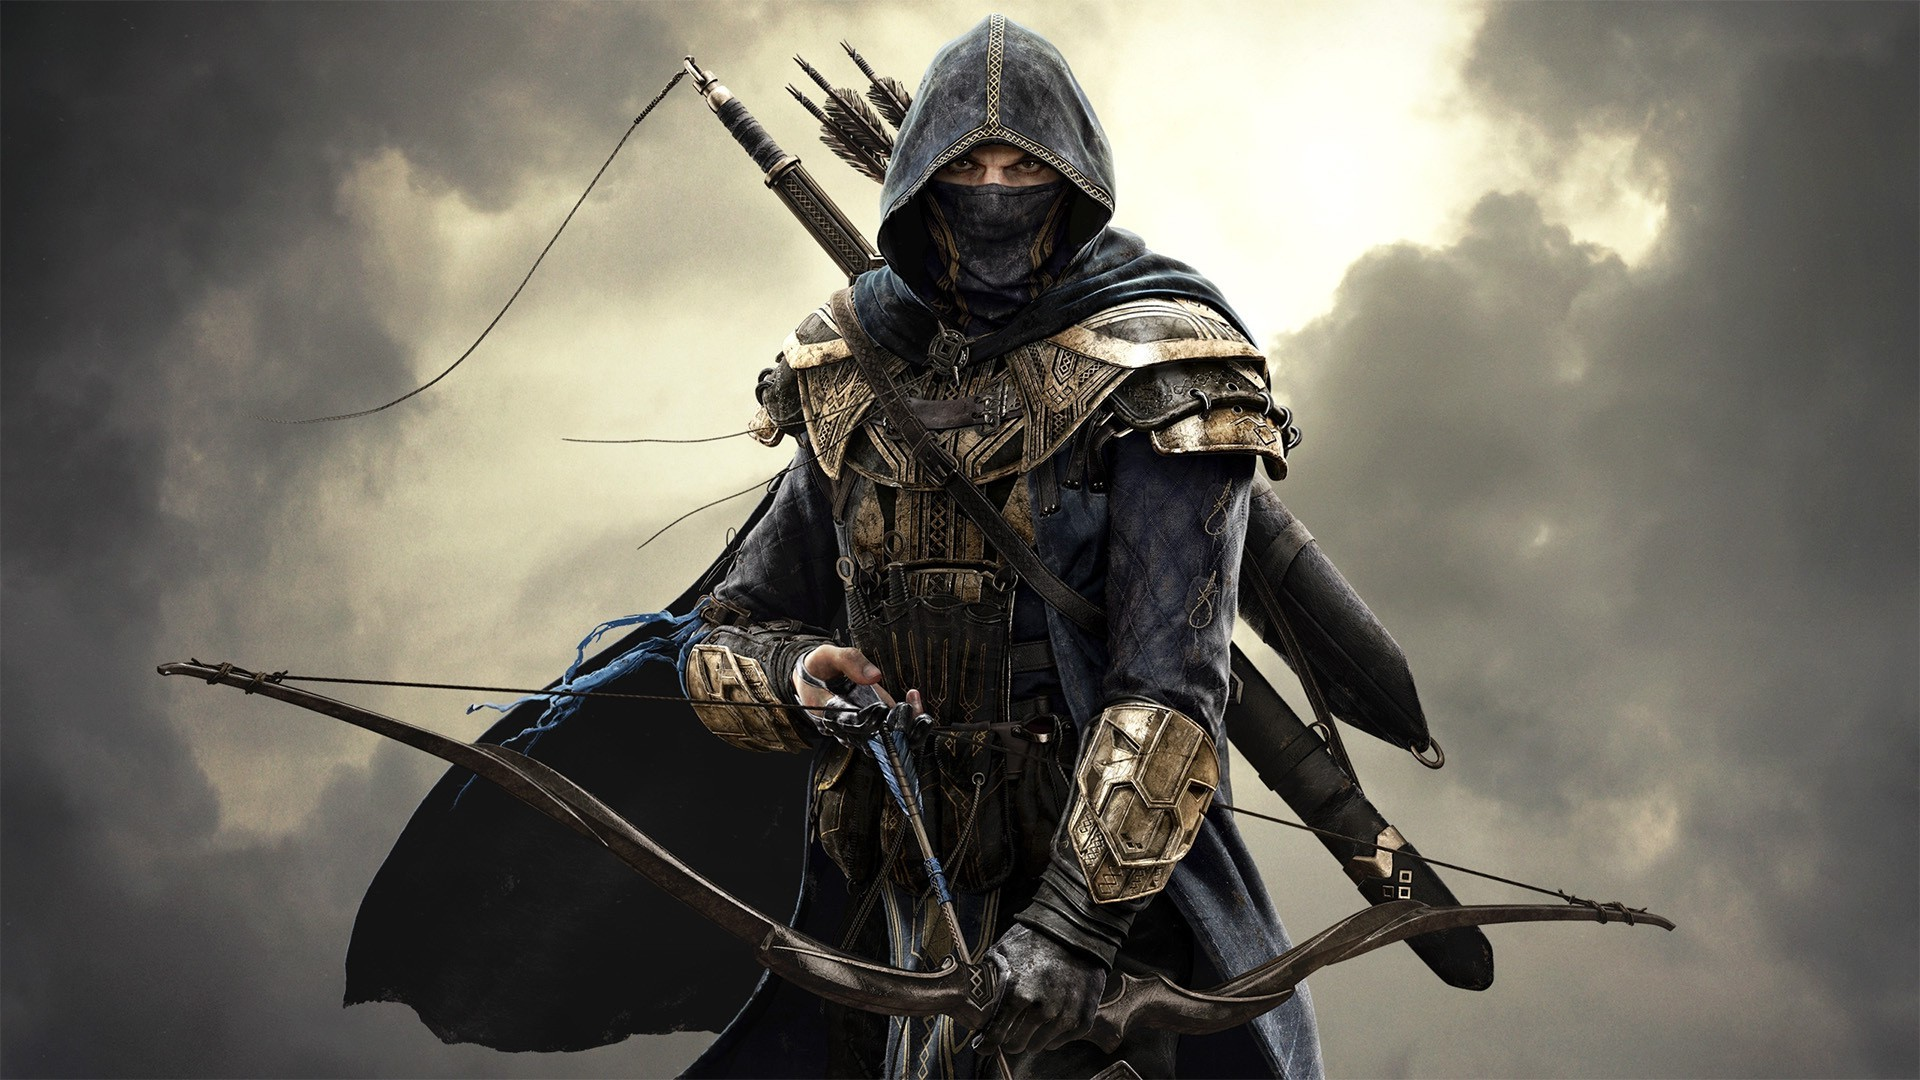
\includegraphics[width=\textwidth]{bretonarcher.png}
\end{figure}